\section{Introduction}
Imagine your brain as an interactive game engine. Just as a game engine generates dynamic virtual environments, complete with rules and physics that players interact with, the brain constructs a model of the real world. This model includes rules (physical laws, social norms), entities (objects, people), and interactions (how things work and relate to each other). We learn to navigate and predict our environment, constantly updating our internal model based on new experiences and information.
This analogy, introduced by \citet{ullmanMindGamesGame2017} extends beyond mere perception, encompassing imagination, dreams, and memory. Each of these cognitive functions can be seen as manifestations of the brain's ability to generate, manipulate, and explore various scenarios and possibilities within its internal model. Dreams and imaginative constructs, while seemingly detached from reality, are composed of the same 'material' as our waking perceptions – they are all products of the brain's simulation capabilities \cite{pearsonHumanImaginationCognitive2019}.
The self, in this view, becomes both a creator and a perceiver of its subjective reality, a reality that, while grounded in the external world, is ultimately shaped by the mind's interpretative and predictive faculties.

In the following, an overview of the fundamental concepts used in this thesis are presented, focusing on program synthesis and its relevance to understanding human cognitive processes. Strengths and limitations of current models are discussed before outlining the approach of overcoming said limitations. FlowCoder \footnote{FlowCoder is available at \url{https://github.com/R1704/master_thesis}} is introduced as a proposed model for program synthesis. A computational model and implementational details are discussed. Two experiments are outlined and their results are analyzed. Finally, improvements and various implications of the model are highlighted.

\subsection{Background}
Traditionally, \acrfull{ai} research has been approached from two general directions. \acrfull{gofai} is based on symbolic reasoning. Symbols have no internal structure but gain significance in relation to other symbols. Models based on formal reasoning are said to be precise and tend to generalize well, yet they are slow and inflexible. Instead, deep-learning relies on distributed vector representations that have a similarity structure and facilitate analogical reasoning, which may be a core function of cognition \cite{bengio2021deep,hofstadter2013surfaces}. These models tend not to generalize well to \acrfull{ood} data and are notoriously data-hungry.
Moreover, composition, systematic generalization (\acrshort{ood}), and abstraction are often argued to be crucial aspects of human cognition \cite{cholletMeasureIntelligence2019, lecun2022path,Fodor_Pylyshyn_1988, hofstadter2013surfaces, boicho2001analogical}, which may be facilitated by a latent innate capacity for the representation and construction of part-whole hierarchies 
\cite{berwickPovertyStimulusRevisited2011,fristonWorldModelLearning2021,hintonHowRepresentPartwhole2021,martinsHowChildrenPerceive2014,raussWhatBottomUpWhat2013,schwartzBehavioralNeuralConstraints2017}.

\paragraph*{Language of Thought}\label{subsubsec:pplot}
\citet{dehaeneSymbolsMentalPrograms2022} posit that human cognition is uniquely characterized by its ability to form symbolic representations and recursive mental structures akin to a \acrfull{lot}, enabling the creation of domain-specific conceptual systems. This cognitive ability allows for the generation of new concepts through the compositional arrangement of existing elements, a process exemplified by the derivation of geometric concepts \cite{alroumiMentalCompressionSpatial2021}. Cognition simplifies complex patterns into mental representations via mental compression, where the complexity of a concept is measured by the length of its mental representation as per the \acrfull{mdl} principle. 

To illustrate, when learning to play chess, rather than remembering as many games as possible, we capture the few rules, through which we can understand and explain all instances of the game.

\begin{figure}[H]
    \centering
    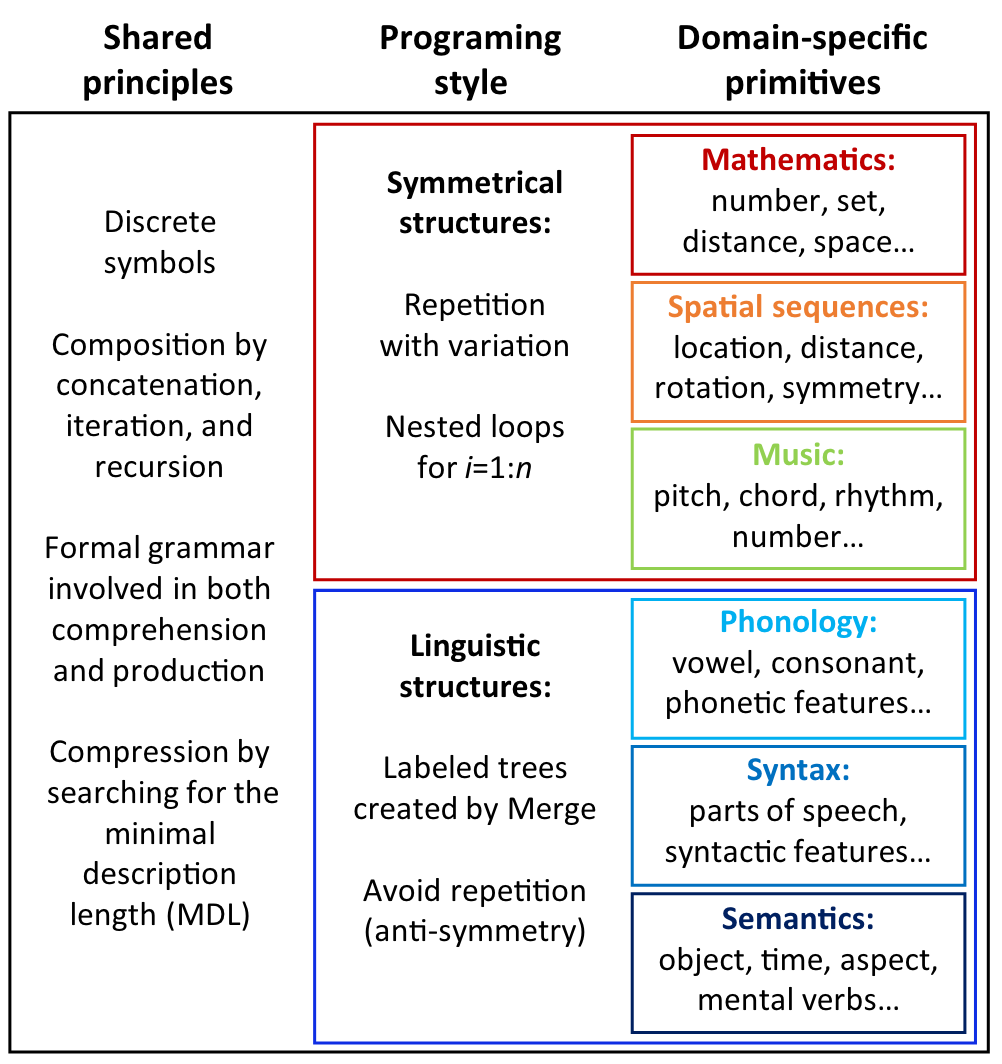
\includegraphics[width=0.7\textwidth]{../img/DSL.png}
    \caption{Human cognition is underpinned by multiple mental \acrfullpl{dsl}. Each language has basic building blocks - primitives which can be programmatically composed to form more complex structures. \citet{dehaeneSymbolsMentalPrograms2022} distinguish between symmetric and asymmetric programming styles. The design principles of these mental languages are shared. They are symbolic, recursive, compositional, use formal grammar, and compress programs by adhering to the minimal description length principle. The diagram was taken from the original paper \cite{dehaeneSymbolsMentalPrograms2022}.}
    \label{fig:DSL}
\end{figure}

Current versions of the \acrshort{lot} posit that the brain implements mechanisms analogous to those found in probabilistic programming languages, enabling it to represent and infer the probabilistic structure of the world \cite{lakeBuildingMachinesThat2017,ruleChildHacker2020}. A program here can be thought of a procedure that generates more examples of the same concept. If a program would represent the concept "animal", it would generate examples such as "giraffe", "zebra", "fish", and so on. Higher-level programs could produce lower-level programs. In this paradigm, the essential aspect of compositionality gives rise to a part-whole hierarchical structure, which facilitates systematic generalization.

\paragraph*{Program Synthesis and Problem Statement}
This computational model of cognition can be formalized as \emph{program synthesis}, where the goal is to automatically construct programs that satisfy a given set of specifications.
Program synthesis involves defining a domain-specific language with a set of primitives and rules, and then searching within this language for a program that satisfies a given set of input-output relations, representing the task at hand. This process is fundamentally about mapping a defined task to an executable program within the constraints of the specified \acrshort{dsl}.

A Domain-Specific Language \( \mathcal{D} \) is defined as a set of syntactic and semantic rules that determine the structure and meaning of valid expressions in the language. Formally, a \acrshort{dsl} can be represented as:
\[ \mathcal{D} = \{ \mathcal{S}, \mathcal{O}, \mathcal{R} \} \]
where \( \mathcal{S} \) is the syntax defining the structure of valid expressions, \( \mathcal{O} \) is the set of operations (or primitives) available in the language, and \( \mathcal{R} \) are the semantic rules that assign meaning to the expressions.

Primitives in the \acrshort{dsl} are the basic operations from which programs are constructed. Each primitive \( o \in \mathcal{O} \) can be thought of as a function:
\[ o: A \rightarrow B \]
where \( A \) is the set of input types and \( B \) is the output type for the primitive.

A task \( x \in X \) in program synthesis is defined as a set of input-output pairs that specify the desired behavior of a program. Formally, a task can be represented as:
\[ x = \{ (x_{in_1}, x_{out_1}), (x_{in_2}, x_{out_2}), ..., (x_{in_n}, x_{out_n}) \} \]
where each pair \( (x_{in_i}, x_{out_i}) \) consists of an input \( x_{in_i} \) and the corresponding desired output \( x_{out_i} \).
The objective of program synthesis is to find a program \( \rho \) within the language \( \mathcal{D} \) that satisfies the task \( x \). Formally, this can be seen as a search problem:
Find \( \rho \in \mathcal{D} \) such that for every \( (x_{in_i}, x_{out_i}) \in x \), \( \rho(x_{in_i}) = x_{out_i} \).

\paragraph*{DreamCoder}\label{subsubsec:dreamcoder}
\acrfull{dc} stands out as a particularly effective model in program synthesis, creating programs from basic primitives and tasks with the goal of developing its own domain-specific language \cite{ellisDreamCoderBootstrappingInductive2021}. It employs an adapted wake-sleep algorithm, initially introduced by \citet{hinton1995wake}, to simultaneously train a generative model and a recognition network. The generative model is tasked with learning a probability distribution across programs, while the recognition network is designed to map tasks to specific programs, facilitating a neurally-guided exploration of the program space. This process leverages the recognition network to implement a parallel search strategy, blending best-first and depth-first searches to prioritize programs based on their probabilities.

The model significantly narrows the search scope by abstracting frequently used sub-routines into more readily accessible concepts, thereby enhancing scalability. This abstraction not only reduces the depth of the search tree but also limits its breadth, with the abstraction phase playing a pivotal role in refactoring subroutines in accordance with the \acrlong{mdl} principle and in the learning of the \acrlong{dsl}.

The tasks addressed by DreamCoder can either be generative, such as image creation, or conditional, like establishing input-output relationships for list sorting. Examples of tasks from various domains are depicted in \autoref{fig:conc_library}(A), while \autoref{fig:conc_library}(B) illustrates the process of learning to sort a list. The figure shows initial primitives on the left, a middle section highlighting the library of learned concepts and the established part-whole hierarchy, and on the right, the ultimate solution employing \texttt{concept15}, which itself incorporates previously abstracted concepts.

\begin{figure}[H]
    \centering
    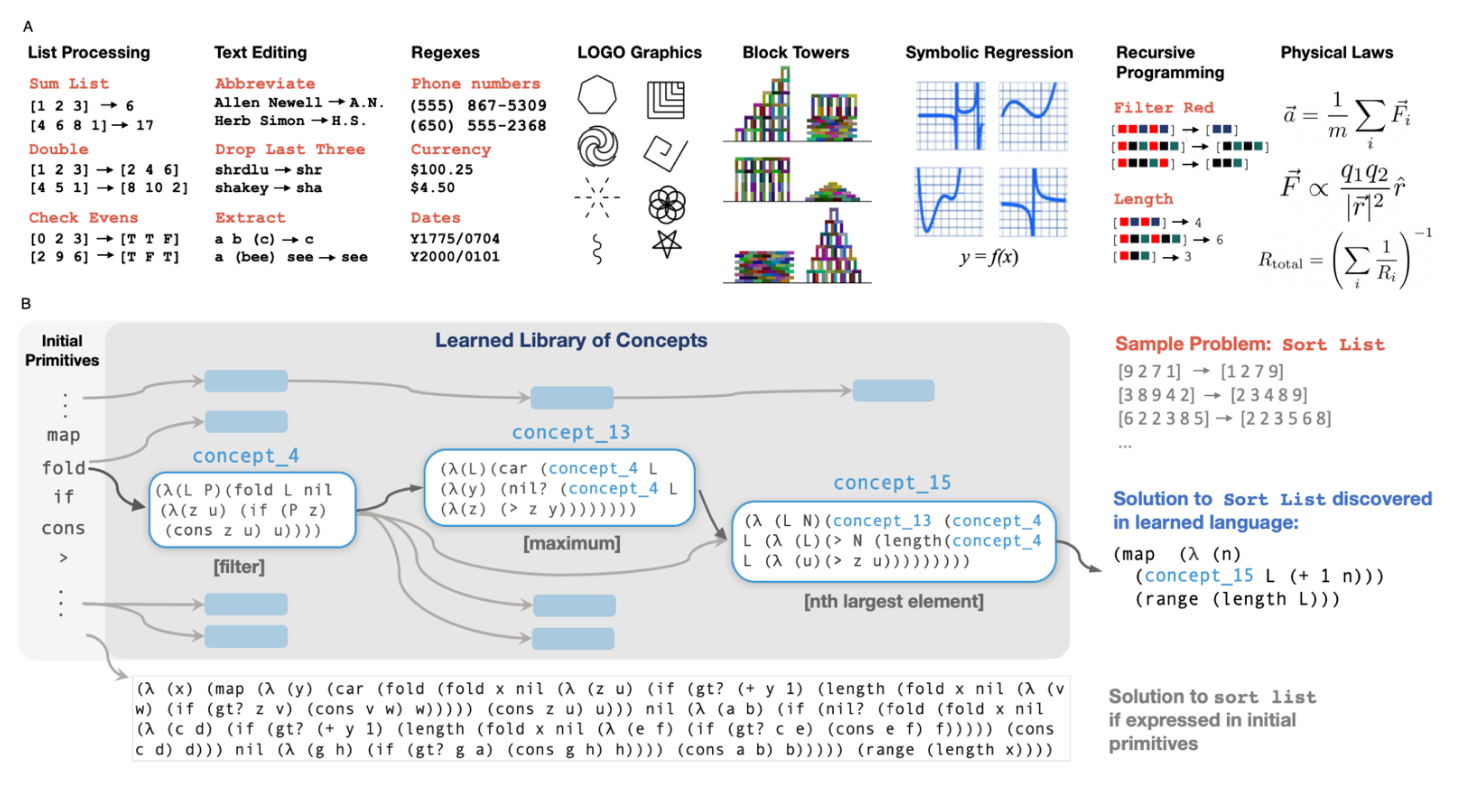
\includegraphics[width=\textwidth]{../img/conc_library.png}
    \caption{(A) Tasks across eight distinct domains. (B) Illustration of the concept library that has been acquired. The left side displays the foundational primitives that are used to construct the concepts shown in the central area. To the right, a task is presented through input-output relationships alongside the derived solution. Below, this solution is reformulated using solely the initial primitives. Image taken with permission from the original paper \cite{ellisDreamCoderBootstrappingInductive2021}.}
    \label{fig:conc_library}
\end{figure}


\paragraph*{DeepSynth}

\citet{fijalkowScalingNeuralProgram2021} propose a framework called "distribution-based search", in which they investigate the difficult problem of searching through a \acrshort{dsl} to find programs matching a specification in a vast hypothesis space.
They introduce DeepSynth \footnote{\url{https://github.com/nathanael-fijalkow/DeepSynth}}, a general-purpose program synthesizer which constructs programs from input-output examples, and a useful framework allowing us to test different models and search methods, which I am using in this project.
The authors discuss different program finding strategies. Specifically, they find that both enumerative search (as in \acrshort{dc}) and sampling are viable strategies, where search is associated with prioritizing quantity, i.e. creating many programs quickly, whereas sampling strategies prioritize quality but may be slower, since resampling may occur. An additional benefit of sampling over search is space efficiency - already created programs don't need to be memorized.
Here, an initial \acrshort{dsl} along with suitable syntactic constraints compile into a \acrfull{cfg}, defining the possible structures of programs within its \acrshort{dsl}. A \acrshort{cfg} consists of a set of production rules that describe how to generate strings from a set of non-terminal and terminal symbols. It is "context-free" because the production rules are applied regardless of the surrounding symbols.
In DeepSynth, a prediction model is used to predict weights for a \acrfull{pcfg}, extending the \acrshort{cfg} by associating probabilities with the production rules. This allows the grammar to not only generate the syntactic structure of a program but also to represent beliefs about the relative plausibility or frequency of different structures \footnote{See appendix \autoref{app:cfg} for a formalization of \acrshortpl{cfg} and \acrshortpl{pcfg}.}. This is similar to DreamCoder's prior, consisting of a library of sub-routines combined with a weight vector. The \acrshort{pcfg} guides the search and inference process towards more likely programs. DreamCoder however, does not specifically use a \acrshort{pcfg}. Both frameworks employ a typed $\lambda$-calculus, hence there are restrictions on program arguments, etc. (syntactical constraints). DreamCoder performs type inference during program generation. To spare computational cost, DeepSynth constructs the \acrshort{cfg} beforehand which in turn increases its size.
\citet{fijalkowScalingNeuralProgram2021} compare different search strategies and show that methods that do not use a machine-learned \acrshort{pcfg} (e.g. \acrfull{dfs}) barely solve any tasks, demonstrating the necessity for better strategies.

\subsection{Limitations}
Although DreamCoder and DeepSynth prove to be successful in synthesizing programs, their methods reveal a foundational limitation: their heavy reliance on syntactical constraints.
While these constraints are undoubtedly vital for ensuring the correctness of generated programs, they do not necessarily guarantee a deep understanding or utilization of semantic relationships within the code. Additionally, \citet{kimCompoundProbabilisticContextFree2019} explain that associating only a scalar per rule misses a lot of information. A distributed representation of the \acrshort{dsl} would therefore be beneficial. We could imagine a program space in which certain symmetries could be leveraged. One could argue e.g. that "\(+\)" is to "\(-\)" as "\(\div\)" is to "\(\times\)". These semantic relationships may be missed in the previously discussed models.

\subsection{Approach}
\paragraph*{Transformers and Self-Attention}
The Transformer architecture, originally introduced in 2017 by \citet{vaswaniAttentionAllYou2017}, has proved to be widely successful in a wide range of applications \cite{wolfTransformersStateoftheArtNatural2020,khanTransformersVisionSurvey2022}. Transformers use self-attention, a mechanism that enables dynamic selection and focus on specific parts of the input, as opposed to treating all parts equally. It effectively allows the network to "attend" to, or give more weight to, certain inputs over others during the processing stage. The self-attention mechanism allows for an understanding of not just the structural arrangement of elements in a sequence (syntax) but also their deeper, contextual relationships (semantics) \cite{wolfram2023chatgpt}. In this thesis I will use this model for a rich representation of programs. However, training the Transformer is difficult from only a few examples. Therefore, I will combine the approach with an amortized sampler, explained in the following.

\paragraph*{GFlowNet}
\acrfullpl{gfn}, introduced by \citet{bengioFlowNetworkBased2021}, are a class of generative models designed to learn to construct compositional objects from a target distribution over complex high-dimensional spaces, particularly where explicit density estimation is challenging and diverse candidates are encouraged. \acrshortpl{gfn} learn a stochastic policy for generating sequences of actions that lead to the construction of a sample. The model generates sequences of actions that build a sample, with the generation frequency of each sample being proportional to an associated reward function.
In other words, \acrshortpl{gfn} are applicable in problems where complex structures are composed from simple building blocks and have been used in molecular composition from atoms \cite{bengioFlowNetworkBased2021}, in grammar induction \cite{Hu_Malkin_Jain_Everett_Graikos_Bengio_2023}, and in Bayesian structure learning \cite{deleuBayesianStructureLearning2022}. The learnt policy becomes an amortized sampler. This means that the extensive training invested in the model results in a system capable of efficiently generating new samples without the need for additional, extensive computation for each new instance. Moreover, the model can be used for offline training, i.e. from data that is not from the observed distribution. This aspect is crucial for \acrshort{ood} generalization and may be the remedy for data-hungry Transformers.

\subsection{Research Question, Aim, Motivation}
In recent advancements, \acrfull{sota} models like \acrlong{dc} have demonstrated proficiency in program synthesis. However, they often lack a semantically rich state representation and heavily rely on search algorithms for constructing programs. This thesis aims to investigate a novel approach by combining the strengths of two distinct architectures: the Transformer and \acrshort{gfn}. The Transformer architecture is known for its ability to learn rich state spaces, albeit with a significant data requirement and limited generalization to \acrlong{ood} tasks. On the other hand, \acrshort{gfn}, with its capability for amortized sampling, presents a promising solution to overcome these challenges. The central hypothesis of this thesis is that the integration of these two architectures could yield a powerful program synthesizer. This synthesizer would be capable of solving tasks with minimal examples, specifically in the list-editing domain. 
Furthermore, theoretical and computational challenges are identified and addressed within the realm of neural program synthesis.

This research explores the potential alignment of the proposed model with the \acrlong{lot} hypothesis, suggesting a programming language-like mental representation underpinning human thought. 
Thus, this research not only aims to address a practical gap in program synthesis but to explore the role of program synthesis in a model of cognition, thereby contributing to the philosophical and psychological understanding of thought, and intelligence. 

\subsection{Scope and Limitations}
The concept of abstraction in program synthesis is necessary for the model to learn its own \acrshort{dsl}. Abstraction effectively narrows the depth of the search tree through program refactoring and identifies common patterns, thereby aiding in generalization. Additionally, abstraction is essential in optimizing for the \acrlong{mdl}, which is a useful inductive bias humans seem to employ \cite{sable-meyerLanguageThoughtMental2022}.
However, in this research, abstraction was not implemented. This decision was primarily guided by time constraints. As a result, I focus on modeling a program synthesizer that solves tasks and on testing its abilities, rather than additionally learning the \acrshort{dsl}. Consequently, it is anticipated that the model will not optimize for parsimonious programs.


% \subsection{\red{Main Contributions}}
% FlowCoder \footnote{Code available at \url{https://github.com/R1704/master_thesis}}.
% % Highlight the significance of your research within the field of AI. Explain how your work contributes to advancing knowledge or addressing the identified research gap. Mention the potential impact of your findings or proposed solutions.
% % The main contributions of this thesis are: 
% % \begin{itemize}
% %     \item I argue that the same multi-scale hierarchies that govern biological organization can be applied to the conceptual realm
% %     \item I develop a method of bayesian program synthesis, using GFlowNet
% %     \item I present the philosophical ramifications
% % \end{itemize}

% % \begin{itemize}
% %     \item novel program synthesizer FlowCoder
% %     \item philosophical ramifications as a model of cognition
% %     \item results 
% %     \item conclusion.
% % \end{itemize}





% I present a novel method for program synthesis and show that systematic generalization is achievable without explicit world models, i.e. without parameterizing a \acrshort{dsl} or \acrshort{pcfg}. Rather, implicit world models in the form of Transformers may be sufficient. I discuss the consequences of the two variants and propose extensions to my model. 